\documentclass[a4paper,12pt]{article}
\usepackage[utf8]{inputenc}
\usepackage[T2A]{fontenc}
\usepackage[russian]{babel}
\usepackage{graphicx}
\usepackage{amsmath,amsfonts,amssymb}
\usepackage{geometry}
\geometry{top=2cm, bottom=2cm, left=2.5cm, right=1.5cm}
\usepackage{indentfirst}
\usepackage{multirow}
\usepackage{booktabs}
\usepackage{caption}
\usepackage{pgfplots}
\pgfplotsset{compat=1.18}
\usepackage{tikz}
\usetikzlibrary{patterns}
\usepackage{setspace}
\onehalfspacing
\usepackage{siunitx} % Для красивых единиц измерения

% Красивые заголовки
\usepackage{titlesec}
\titleformat{\section}{\Large\bfseries\sffamily}{\thesection}{1em}{}
\titleformat{\subsection}{\bfseries\sffamily}{\thesubsection}{1em}{}
\titleformat{\subsubsection}{\bfseries\sffamily}{\thesubsubsection}{1em}{}

% Для имитации рукописного шрифта в титуле (опционально)
\usepackage{aurical}
\usepackage{color}

\begin{document}

% Титульный лист
\begin{titlepage}
    \begin{center}
        % Верхняя часть с названием вуза
        \textbf{МОСКОВСКИЙ ФИЗИКО-ТЕХНИЧЕСКИЙ ИНСТИТУТ} \\
        \textbf{(НАЦИОНАЛЬНЫЙ ИССЛЕДОВАТЕЛЬСКИЙ УНИВЕРСИТЕТ)}
        \\[1cm]

        
        % Название факультета (чуть меньше)
        {\large Физтех-школа аэрокосмических технологий}
        \\[3.5cm]

        % Самое большое — полное название работы
        {\Huge \textbf{Исследование колебаний жидкости в канале}}
        \\[0.5cm]

        % Блок с именами и группами (выравнивание по правому краю)
        \begin{flushright}
            \begin{tabular}{l l}
                Копышова Валентина Олеговна & Б03-3046 \\
                Ларькин Глеб Сергеевич & Б03-301а \\
                Дай Сюй                  & Б03-3046 \\
                Ордоньес Эррера Хулио Себастьян & Б03-304б \\
                Бобровский Дмитрий Андреевич & Б03-305 \\
            \end{tabular}
        \end{flushright}

        \vfill

        % Нижняя часть
        {\large Долгопрудный, 2026 г.}
    \end{center}
\end{titlepage}

\tableofcontents
\newpage

\section{Введение}

\section{Теоретическая часть}
Далее приведен вывод по В.В. Кривецу.

\subsubsection*{Поставновка задачи}
Рассматривается кювета, заполненная двумя несмешивающимися жидкостями,
колеблющаяся в поле тяготения Земли. Область течения задаётся как
$z \in [-h_2,\, h_1]$. Положение границы раздела жидкостей описывается
функцией $z = \xi(x, t)$.

Принятые приближения:
\begin{itemize}
    \item Рассматриваются малые колебания: $a\kappa \ll 1$,
          $\xi\kappa \ll 1$, где $a$ — амплитуда, $\kappa$ — волновое число.
    \item Течение потенциально (безвихревое): $\nabla \times \mathbf{u} = 0$,
          поэтому $\mathbf{u} = \nabla\varphi$.
    \item Нелинейным членом $(\mathbf{u} \cdot \nabla)\mathbf{u}$
          пренебрегаем ввиду малости колебаний.
\end{itemize}

Для жидкости снизу: плотность $\rho_2$, давление $P_2$, потенциал скорости $\varphi_2$.

Для жидкости сверху: плотность $\rho_1$, давление $P_1$, потенциал скорости $\varphi_1$.


Из условия несжимаемости и потенциальности течения следует уравнение Лапласа:
\begin{equation}
    \Delta \varphi = 0.
\end{equation}

Запишем уравнение Бернулли:
\begin{equation}
    \frac{\partial \varphi}{\partial t} + \frac{P}{\rho} + gz = \mathrm{const}.
    \label{eq:bernoulli}
\end{equation}

\subsubsection*{Граничные условия}

Условие непротекания:
\begin{equation}
    \left.\frac{\partial \varphi}{\partial z}\right|_{z=\pm h_{1,2}} = 0.
\end{equation}

Непрерывность нормальной компоненты скорости:
\begin{equation}
    \left.\frac{\partial \varphi_1}{\partial z}\right|_{z=\xi}
    = \left.\frac{\partial \varphi_2}{\partial z}\right|_{z=\xi}
    = \frac{\partial \xi}{\partial t}.
    \label{eq:kinematic}
\end{equation}

Непрерывность давления:
\begin{equation}
    P_1\big|_{z=\xi} = P_2\big|_{z=\xi}.
    \label{eq:dynamic}
\end{equation}

\subsection*{Решение}

Ищем решение в виде:
\begin{equation}
    \varphi(x, z, t) = T(t)\, X(x)\, Z(z).
\end{equation}

Подстановка в уравнение Лапласа даёт задачу Штурма–Лиувилля:
\begin{equation}
    \frac{X''}{X} = -\frac{Z''}{Z} = -\kappa^2,
\end{equation}
откуда $X'' + \kappa^2 X = 0$ и $Z'' - \kappa^2 Z = 0$.

С учётом условий непротекания на стенках решения, удовлетворяющие
граничным условиям, имеют вид (подробнее см.~Ландау, Лифшиц,
«Гидродинамика», \S\,4):
\begin{align}
    \varphi_1 &= T_1(t)\,\cos(\kappa x)\,
                 \cosh\!\bigl(\kappa(z - h_1)\bigr), \label{eq:phi1} \\
    \varphi_2 &= T_2(t)\,\cos(\kappa x)\,
                 \cosh\!\bigl(\kappa(z + h_2)\bigr). \label{eq:phi2}
\end{align}
Использование $\cosh$ вместо $e^{\pm\kappa z}$ обеспечивает автоматическое
выполнение условия непротекания на дне и потолке кюветы.

Подставляя \eqref{eq:phi1}, \eqref{eq:phi2} в кинематическое условие
\eqref{eq:kinematic} при $z = \xi \approx 0$ (линеаризация):
\begin{equation}
    -T_1\,\sinh(\kappa h_1) = T_2\,\sinh(\kappa h_2),
\end{equation}
откуда:
\begin{equation}
    T_2 = -\frac{T_1\,\sinh(\kappa h_1)}{\sinh(\kappa h_2)}.
    \label{eq:T2}
\end{equation}

Из динамического условия \eqref{eq:dynamic} с помощью уравнения Бернулли
\eqref{eq:bernoulli}, дифференцируя по $t$ и используя \eqref{eq:T2}:
\begin{equation}
    -T_1\kappa =
    \frac{\ddot{T}_1\bigl(\rho_1\coth(\kappa h_1)
    + \rho_2\coth(\kappa h_2)\bigr)}{(\rho_2 - \rho_1)\,g}.
\end{equation}

Полагая $T_1 \propto e^{i\omega t}$, получаем дисперсионное соотношение:
\begin{equation}
    \omega^2 = \frac{(\rho_2 - \rho_1)\,g\,\kappa}
                    {\rho_1\coth(\kappa h_1) + \rho_2\coth(\kappa h_2)}.
    \label{eq:dispersion}
\end{equation}

В предельном случае $\rho_1 \to 0$ (одна жидкость со свободной поверхностью):
\begin{equation}
    \omega^2 = g\kappa\tanh(\kappa h_2),
    \qquad \kappa = \frac{n\pi}{L}, \quad n = 1, 2, \ldots
    \label{eq:dispersion_simple}
\end{equation}
(см.~формулу~(4.15) в учебнике).

\newpage
\section{Экспериментальная установка и методика}

Ниже представлена схема экспериментальной установки:
\begin{figure}[h!]
  \centering
  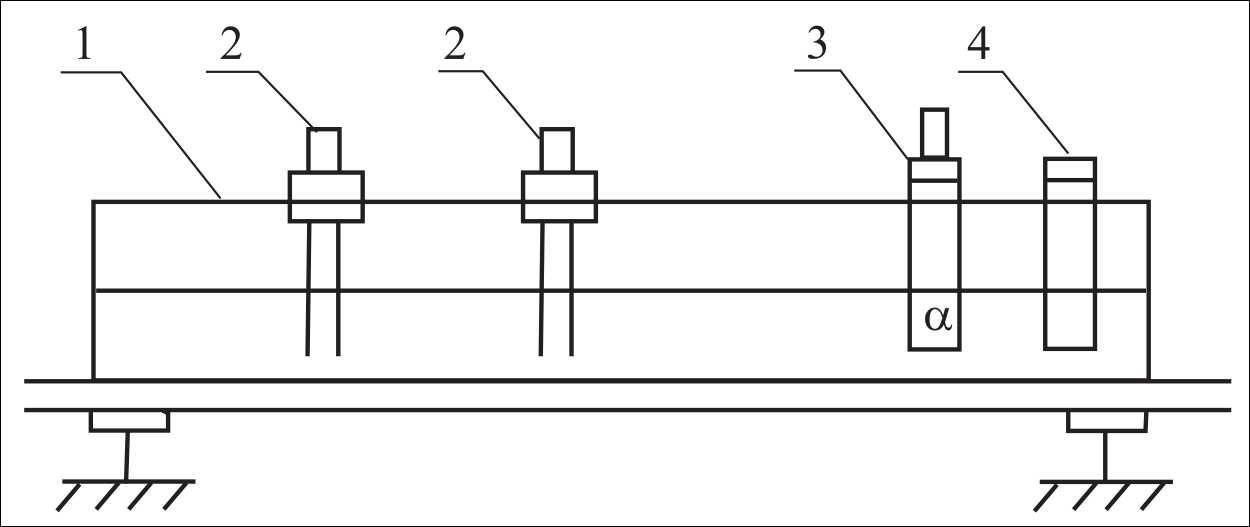
\includegraphics[width=0.7\textwidth]{photoes/sheme.png}
  \caption{Схема экспериментальной установки}
  %\label{fig:label}
\end{figure}


Установка состоит из канала прямоугольного сечения (1), изготовленного из оргстекла, на котором закреплён динамик (3), выполняющий роль волногенератора, и две салазки с щупами (2) для измерения уровня жидкости. 

При изменении уровня жидкости меняется сопротивление в цепи, и на осциллограф подаётся напряжение, пропорциональное измеренному уровню. 


\section{Ход работы}
Сначала были зарегистрированы параметры лабораторной установки. Расстояние от генератора волн до отражающей стенки кюветы составило $L = 144$ см, а глубина воды — $h = 3.4$ см. Используя эти данные и формулу (14), рассчитали частоты, при которых в кювете возникают стоячие волны.

При установке каждой из рассчитанных частот датчики амплитуды располагали следующим образом: первый датчик размещали в области максимального изменения амплитуды волны, а второй перемещали до тех пор, пока регистрируемый им сигнал не становился равным по амплитуде сигналу первого датчика, но сдвинутым по фазе на половину периода. Таким образом обеспечивалось расположение датчиков в соседних пучностях, и расстояние между ними соответствовало половине длины волны. Данная процедура повторялась для каждой частоты.

Впоследствии, используя формулу (14), построили график зависимости частоты \(\omega\) от волнового числа \(\kappa\). На рисунке 2 представлено сравнение теоретической кривой с экспериментальными данными.

Наконец, применив преобразование Фурье к данным, полученным с осциллографа, получили частотный спектр волн, генерируемых в кювете, как показано на рисунке 3. Частота с максимальной амплитудой соответствует частоте генератора \(f = 3.3\) Гц.

\newpage
\section{Результаты измерений и обработка результатов}
При анализе формулы (14) видно, что при глубине $h << L$ и малых волновых числах, что выполняется в нашей работе, ожидается практически линейная зависимость $w(\kappa)$, тк при малых значениях x выполнено $tanh x = x + o(x^3)$. 

Ниже представлена теоретическая зависимость и экспериментальные точки:
\begin{figure}[h!]
  \centering
  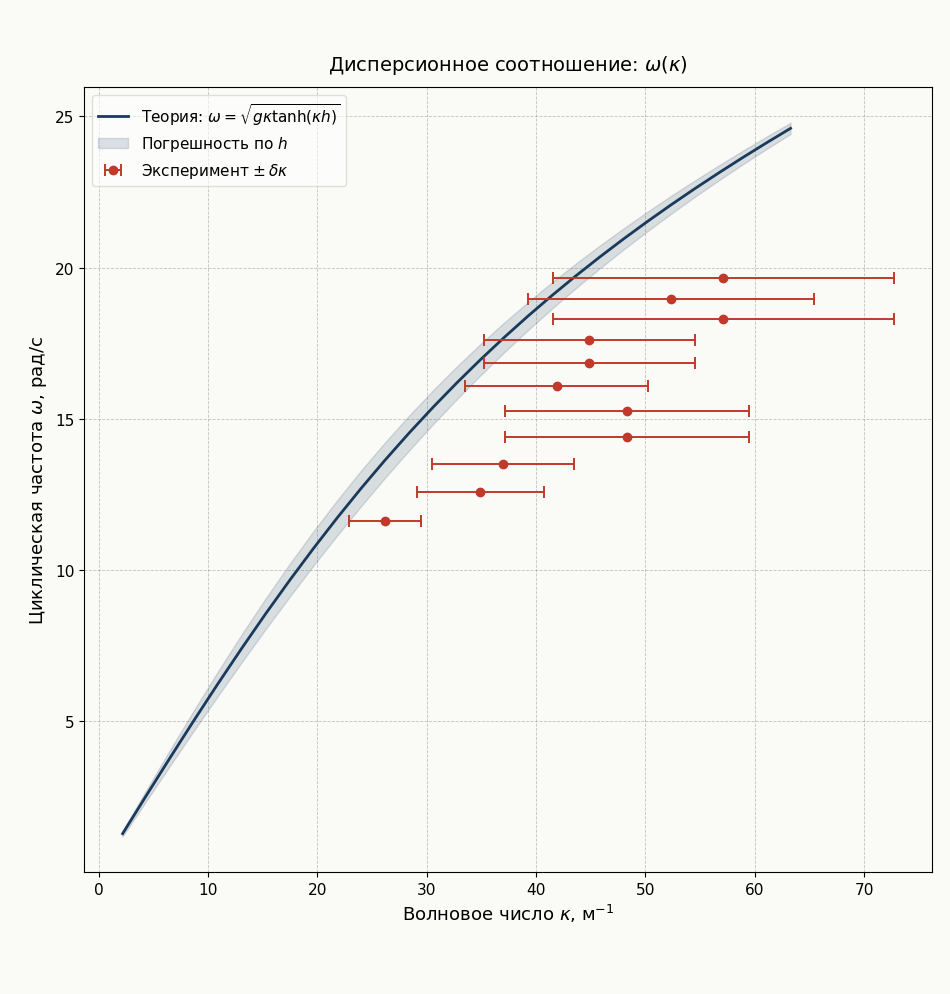
\includegraphics[width=1.0\textwidth]{photoes/w(k).png}
  \caption{Зависимость волнового числа от частоты}
  %\label{fig:label}
\end{figure}

Также, как уже писалось выше, в работе исследовался спект волнового генератора, для этого делалось преобразование Фурье от функции напряжения от времени $U(t)$. Ожидается, что будет наблюдаться единственный пик на собственной частоте, то есть на частоте генератора $3.3$ Гц.
\begin{figure}[h!]
  \centering
  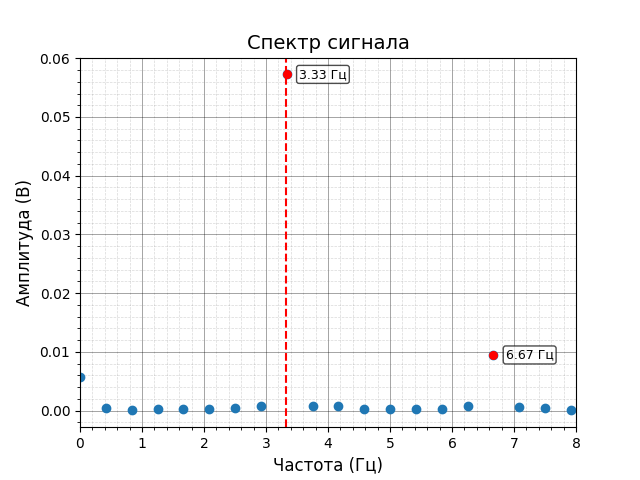
\includegraphics[width=0.8\textwidth]{photoes/furie.png}
  \caption{Преобразование Фурье от функции напряжения от времени $U(t)$}
  %\label{fig:label}
\end{figure}

\section{Обсуждение результатов и выводы}
На графике с преобразованием Фурье пик действительно попадает на частоту генератора 3.3 Гц. Также наблюдается пик 6.6 Гц, те удвоенная частота генератора, а также пик около нуля. 

- Пик в 6.6 Гц, как нам кажется, связан с неидеальностью генератора.

- Пик в окрестности нуля, вероятно, связан с колебаниями самой установки.

Так как генератор работает на двух частотах, а не на одной (а теория выведена для идеального генератора), из-за интерференции двух создаваемых волн минимальное расстояние между двумя равными высотами волн уменьшается, что ведет к наблюдаемому увеличению волновых чисел относительно теоретически предсказанных при заданной частоте. Стоит отметить, что неидельность генератора делает измерение длины волны невозможным, так как не очень понятно, что подразумевается под длиной волны интерференционной картины. Поэтому теоретическая оценка дает лишь оценку по порядку величины.

Можно значительно увеличить точность измерений, измеряя не половину длины волны, а несколько длин волн, что позволит при помощи усреднения получить характерный размер системы, который может пониматься под длиной волны интерференционной картины. 

\end{document}